% CVPR-style survey (course final report)
% Template style from https://github.com/cvpr-org/author-kit
\documentclass[10pt,twocolumn,letterpaper]{article}

\usepackage[pagenumbers]{cvpr}
\usepackage{graphicx}
\usepackage{amsmath,amssymb}
\usepackage{booktabs}
\usepackage{xspace}

\definecolor{cvprblue}{rgb}{0.21,0.49,0.74}
\usepackage[breaklinks,colorlinks,allcolors=cvprblue]{hyperref}

\def\confName{CVPR}
\def\confYear{2026}

\title{Machine Unlearning in Computer Vision:\\ Methods, Benchmarks, and Robustness}

\author{
Student Author\\
Computer Vision Course Final Survey\\
{\tt\small anonymous@university.edu}
}

\begin{document}
\maketitle

\begin{abstract}
Machine unlearning (MU) aims to remove the influence of specific data points, classes, or semantic concepts from trained models without full retraining. In computer vision, this capability is increasingly required for privacy compliance, copyright protection, and safety alignment across face recognition, medical imaging, text-to-image generation, and vision-language assistants. This survey organizes 2020--2026 vision unlearning research along four axes---targets, strategies, architectures, and evaluation---covering discriminative classifiers (CNNs and Vision Transformers), diffusion models, and vision-language models (VLMs). We highlight a fundamental gap between discriminative parameter-space forgetting and generative concept erasure in entangled latent spaces, and show that many methods achieve only superficial suppression under adversarial probing. We conclude with open challenges toward verifiable and robust vision unlearning.
\end{abstract}

\section{Introduction}

Computer vision is not a peripheral application of machine unlearning; it is one of the domains where technical difficulty and societal impact concentrate most sharply. Unlike text-only models, vision systems process high-dimensional perceptual signals whose information is distributed across spatial features, cross-modal alignments, and generative latent spaces. The ``right to be forgotten'' established by GDPR and CCPA requires that deployed models no longer encode a subject's identity, medical characteristics, or copyrighted style after a deletion request. Meanwhile, text-to-image systems must suppress celebrity portraits, NSFW content, and proprietary IP characters, and vision-language models must disentangle sensitive image--text associations. These needs map onto sample/class removal in classification, identity erasure in person re-identification, concept suppression in diffusion models, and cross-modal decoupling in multimodal models~\cite{bourtoule2021,safavigerdini2026}.

From an industrial perspective, vision unlearning is no longer a purely academic setting. Face recognition services must delete memory of a user's appearance after consent withdrawal; medical imaging systems must erase training traces of specific exams; open-source text-to-image communities must remove styles or characters upon copyright complaints. Zhang~\etal~\cite{zhang2023review} provide terminology and taxonomy for general MU, but vision exhibits more complex failure modes: a model may ``refuse'' a concept in explicit outputs while retaining recoverable cues in latent representations or conditional generation. Bourtoule~\etal~\cite{bourtoule2021} formalized MU at IEEE S\&P 2021 and proposed shard-based approximate exact forgetting. The vision community rapidly extended this paradigm to classifiers, generators, and multimodal foundation models. The CVPRW 2026 survey of Safavigerdini~\etal~\cite{safavigerdini2026} charts the trajectory from discriminative erasure to generative concept suppression and robust unified frameworks, while the ICCV 2025 HUB benchmark~\cite{moon2025hub} marks a shift from ``can we erase'' to ``can erasure survive multi-dimensional threats.''

\paragraph{Problem formulation.}
Let $f_\theta$ be trained on $\mathcal{D}$, with forget set $\mathcal{D}_f\subset\mathcal{D}$ and retain set $\mathcal{D}_r=\mathcal{D}\setminus\mathcal{D}_f$. MU seeks parameters $\theta'$ such that $f_{\theta'}$ behaves as if $\mathcal{D}_f$ were never seen, preserves utility on $\mathcal{D}_r$, and updates at far lower cost than retraining from scratch~\cite{bourtoule2021}. Exact unlearning requires statistical indistinguishability from a model retrained only on $\mathcal{D}_r$; approximate unlearning relaxes this guarantee for computational feasibility~\cite{zhang2023review}. In vision practice, exact unlearning is largely restricted to small classifiers, whereas generative foundation models almost always use approximate or heuristic concept suppression. Deletion requests themselves differ: some remove a single user sample, others an entire class label, and others a semantic concept that is not a closed class (e.g., a painting style or fictional character). Unclear target definitions make evaluations incomparable~\cite{zhang2023review}, which motivates stating a four-axis taxonomy before reviewing methods.

\paragraph{Scope and positioning.}
This survey focuses on vision-specific work from 2020--2026, primarily from CVPR, ICCV, NeurIPS, IEEE S\&P, WACV, and arXiv. Pure LLM unlearning is included only when adapted to VLMs. Relative to~\cite{safavigerdini2026}, we emphasize evaluation and robustness: not only method taxonomies, but which metrics can certify that knowledge has truly been removed. Relative to general MU surveys~\cite{zhang2023review}, we do not attempt full-discipline coverage and instead concentrate on three vision architectures and their cross-cutting challenges. The paper contains no original experiments; claims are traceable to the cited literature.

\section{Taxonomy and Architectures}

\subsection{Four-Axis Taxonomy}

Following~\cite{safavigerdini2026}, we organize the literature along four axes (Fig.~\ref{fig:taxonomy}). The first axis is the \emph{forgetting target}: sample-level (single images), class-level (entire labels), or concept-level (styles, identities, NSFW attributes). The second is the \emph{implementation strategy}: data reorganization (sharding, partitioning), model manipulation (gradient updates, weight editing, neuron suppression), or inference-time intervention (activation steering, null-space projection). The third is the \emph{architecture scope}: discriminative (CNN, ViT, Swin), generative (DDPM, Flow Matching, Stable Diffusion), or multimodal (CLIP- and LLaVA-style VLMs). The fourth is the \emph{evaluation protocol}, which should jointly measure forgetting efficacy, utility retention, privacy guarantees, and computational efficiency. Cross-products of these axes provide a skeleton for literature search and evidence mapping: a method is best understood as a target--strategy--architecture--evaluation combination rather than as an isolated acronym.

\begin{figure}[t]
\centering
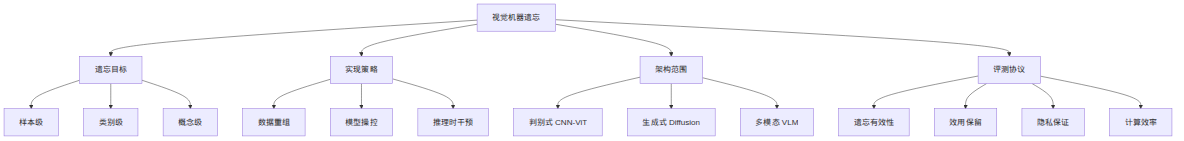
\includegraphics[width=\linewidth]{taxonomy-tree.png}
\caption{Four-axis taxonomy of machine unlearning for vision: targets, strategies, architectures, and evaluation.}
\label{fig:taxonomy}
\end{figure}

\subsection{Architectural Mechanisms}

The three architecture families differ in forgetting mechanisms. Discriminative models primarily operate on decision boundaries and feature geometry; the goal is usually to change the separability of specific samples or classes in representation space. Zhao~\etal~\cite{zhao2026vit} show that Vision Transformers, with global context modeling, often retain higher utility after unlearning than CNNs, whereas CNNs are more compatible with gradient-style methods. Discussing an ``optimal'' unlearning algorithm therefore presupposes the representation biases of the host architecture.

Generative diffusion models encode concepts largely in cross-attention layers, where text embeddings are projected into visual features via $W_k$ and $W_v$. Consequently, ESD~\cite{gandikota2023esd} and UCE~\cite{gandikota2024uce} prioritize editing cross-attention rather than the full U-Net. Cross-attention is the primary but not sole carrier of concept memory: U-Net denoising trajectories, text-encoder embeddings, and classifier-free guidance can all act as residual channels. This explains why later methods explore complementary weight editing, neuron suppression, and inference-time intervention.

VLMs must handle entanglement among vision encoders, text encoders, and fusion decoders. Lin~\etal~\cite{lin2026vlm} show that suppressing text-side outputs alone does not guarantee that residual visual associations are unrecoverable. Visual features often encode object- and attribute-level cues before entering language space, while the language decoder can reinforce those cues during generation. The core difficulty is therefore not deleting a single training example, but interrupting a cross-modal reinforcement loop. Understanding these mechanistic differences is a prerequisite for avoiding naive transplantation of LLM unlearning recipes into vision.

\begin{figure*}[t]
\centering

\includegraphics[width=0.95\textwidth]{research-timeline.png}
\caption{Research timeline of vision machine unlearning (2020--2026), from formalization to benchmarks and robustness.}
\label{fig:timeline}
\end{figure*}

Fig.~\ref{fig:timeline} summarizes key milestones from 2020 to 2026: formalization and shard-based exact forgetting; emergence of ESD/UCE and SCRUB; mass concept erasure and adversarial robustness; multi-dimensional benchmarks such as HUB; and systematic studies of ViT and VLM unlearning.

\section{Discriminative Vision Unlearning}

\subsection{Exact and Approximate Forgetting}

Exact unlearning is represented by Bourtoule~\etal~\cite{bourtoule2021}, who shard training data across submodels to reduce the cost of individual deletions. For large vision classifiers, fully exact unlearning remains impractical, so research centers on approximate methods. SCRUB~\cite{kurmanji2023scrub} combines gradient ascent on the forget set with retain-set distillation to balance forgetting and utility. Projected-gradient unlearning applies updates orthogonal to the subspace spanned by retain-set gradients, reducing interference with unrelated classes; guided loss-increasing objectives use feature-distance and classification guidance to avoid utility collapse under naive ascent. Boundary unlearning further shifts the operation from parameters to decision boundaries and, in some settings, reports order-of-magnitude speedups over retraining.

From an evaluation perspective, Zhao~\etal~\cite{zhao2026vit} provide a landmark ViT study. Under a unified protocol comparing ViT and Swin across model capacities, dataset scales, and single-round versus continual unlearning, they find systematic differences in how Transformers memorize training data relative to CNNs. Algorithms designed for CNNs therefore often transfer poorly. Attention-guided contrastive variants further suggest that architecture specialization will remain a major trend. Marasco~\etal~\cite{marasco2026} argue that unlearning should be treated as a lifecycle capability---covering deployment, updates, and audits---rather than a one-shot post-training patch.

\subsection{Representation- and Knowledge-Level Forgetting}

Editing output logits is often insufficient to remove internal memory. Representation-level methods surveyed in~\cite{safavigerdini2026} exploit Neural Collapse geometry, projecting forget-class features toward the origin in an equiangular tight frame, or impose sparsity and orthogonality constraints on filters to disentangle class-specific representations. Companion metrics such as representation unlearning scores based on centered kernel alignment (CKA) compare forgotten models to gold-standard retrained models at a finer grain than accuracy. Complementary parameter-localization methods identify Markov-blanket subsets or reinitialize highly sensitive parameters, reflecting the view that efficiency depends on locating low-dimensional structures that carry the target information rather than updating the entire network indiscriminately. These approaches push discriminative unlearning from ``outputs are inseparable'' toward ``representations are unrecoverable,'' yet statistical guarantees remain largely confined to closed-set classification and do not transfer readily to open-semantic generative models.

\subsection{Specialized Vision Scenarios}

Face and person-centric tasks refine forgetting into instance-level requirements. Benchmarks such as MUFAC require forgetting specific identities while preserving age and gender estimation, which is substantially harder than CIFAR class deletion~\cite{safavigerdini2026}. This matches product logic: after deleting a user's face, platforms may still need non-identity analytics. Person re-identification methods that shift forgotten features into non-retrievable regions impose a stronger constraint of post-forgetting non-retrievability. Related applications, such as purifying reinforcement-learning policies of backdoors, show that unlearning also serves security repair. Across these settings, the forget object is rarely an i.i.d.\ sample; it is a composite semantic structure (identity, attributes, behavioral policy). Discriminative vision unlearning is therefore as much about defining what to retain versus delete as about optimization algorithms.

\section{Concept Erasure in Diffusion Models}

\subsection{Fine-Tuning versus Closed-Form Editing}

Erased Stable Diffusion (ESD)~\cite{gandikota2023esd} aligns the noise prediction of a target concept with a neutral prompt so that the denoising trajectory avoids undesirable semantics, establishing a lasting baseline. Unlike full U-Net fine-tuning, ESD highlights cross-attention as a structural hub for concepts, shaping subsequent method design. Unified Concept Editing (UCE)~\cite{gandikota2024uce} casts cross-attention weight modification as a closed-form optimization that can suppress a target concept while protecting non-target outputs in a single update, lowering the compute barrier for urgent online deletion requests.

For scalability, MACE~\cite{lu2024mace} combines closed-form refinement with per-concept LoRA adapters and advances erasure capacity to about one hundred concepts; related adapters with dual-level orthogonality constraints mitigate crosstalk under multi-concept erasure. Selective Amnesia-style methods import elastic weight consolidation ideas to protect parameters critical to retained concepts. Differential-vector and related training-free approaches indicate that concept erasure is expanding from Stable Diffusion-specific recipes toward broader generative paradigms such as Flow Matching~\cite{safavigerdini2026}. Overall, fine-tuning typically erases more thoroughly but incurs compute cost and collateral damage; closed-form and training-free routes excel in efficiency and deployability yet are more fragile under strong attacks~\cite{moon2025hub}.

\subsection{Neuron-Level and Latent Interventions}

Beyond weight editing, researchers localize concepts at finer granularity. Sparse autoencoders decompose text-encoder activations into interpretable units that can be selectively suppressed~\cite{safavigerdini2026}. Prototype-guided erasure clusters latent differences into concept prototypes and injects them as negative conditions under classifier-free guidance. Corrector-style methods detect target semantics in intermediate generations and switch to concept-removal attention for on-the-fly intervention. Such methods are especially precise for narrow concepts (specific IP characters, individual celebrities) that occupy relatively separable directions in embedding space.

Broad-concept erasure remains difficult. Categories such as NSFW or violence have diverse visual forms and flexible textual expressions; a single prototype or neuron suppression rarely covers all variants. Erasing a narrow concept can also damage shared super-types (e.g., people in general), creating a structural tension between erasure and fidelity~\cite{safavigerdini2026}. Consequently, concept erasure should not be judged solely by FID or CLIP scores under standard prompts; collateral effects on neighboring semantics must be reported---a motivation for benchmarks that stress implicit prompts and bias amplification~\cite{moon2025hub}.

\subsection{Realistic Evaluation Constraints}

Concept erasure cannot be evaluated only under standard text prompts. White-box protocols that learn embeddings or invert latents show that concept recreation rates of advanced methods can exceed 90\%~\cite{moon2025hub,safavigerdini2026}. HUB~\cite{moon2025hub} covers faithfulness, alignment, pinpoint-ness, multilingual robustness, attack robustness, and efficiency, and finds that no single method leads on all axes. Continual-erasure suites further require that sequential removal of multiple concepts preserve stable generation of retained concepts. The emerging consensus is that the field has moved from ``can we produce clean images'' to ``can erasure persist under adversarial, multilingual, and continual-update conditions.''

\section{Vision-Language Model Unlearning}

\subsection{Method Families}

Lin~\etal~\cite{lin2026vlm} organize VLM unlearning into four families that unify previously scattered practices from LLM and multimodal communities. Full-parameter fine-tuning transplants gradient ascent and negative preference optimization to end-to-end VLMs; it is expressive but costly and prone to damaging general capability. Vision-encoder fine-tuning updates only $\theta_v$ and is often more effective for discriminative probes (e.g., whether an object is present), suggesting that visual concept memory is heavily rooted in the encoder~\cite{lin2026vlm}. Selective-parameter updates locate critical layers or modules to reduce interference; inference-time interventions apply activation masks or neuron edits with frozen weights, offering lightweight but less durable forgetting. Cross-modal decoupling objectives separate image--text associations at training time, while hyperbolic alignment calibration relocates forgotten concepts onto other branches of a semantic hierarchy. Collectively, these lines show that VLM unlearning is not a simple repetition of LLM unlearning: it must handle bidirectional dependence between visual grounding and language description.

\subsection{Cross-Modal Entanglement and Evaluation}

VLM unlearning must simultaneously satisfy forgetting, retention, and general-capability goals~\cite{lin2026vlm}. Models may correctly refuse a target concept under direct descriptive prompts yet recover associations under paraphrases, contextual cues, or discriminative questioning. In-distribution retraining and out-of-distribution transfer attacks further indicate that many methods \emph{hide} rather than \emph{erase}: an adversary with a few same-distribution samples---or even semantically related but distributionally different auxiliaries---can reactivate target knowledge~\cite{lin2026vlm}. For VLMs deployed in medical or legal settings, forgetting that cannot survive subsequent fine-tuning or prompt engineering is questionable as compliance evidence. Evaluation must therefore go beyond single-prompt accuracy to multi-prompt variants, retraining recovery rates, and cross-modal probes. We view VLMs as among the most challenging vision-unlearning subareas for the next several years, not only because of scale but because forgetting evidence is hard to observe in a single modality.

\section{Robustness, Attacks, and Defenses}

\subsection{Suppression versus Erasure}

A central consensus in recent vision unlearning literature is the distinction between output suppression and knowledge erasure. In diffusion models, concept revival shows that subsequent fine-tuning on unrelated data can resurrect erased semantics~\cite{safavigerdini2026}; in VLMs, contextual and retraining attacks recover forgotten associations with few samples~\cite{lin2026vlm}. White-box results indicate that standard-prompt evaluation severely overestimates erasure quality~\cite{moon2025hub}. Robustness is therefore not an optional add-on but a necessary condition for claiming that unlearning has occurred. From a legal and product perspective, proving that a model no longer emits sensitive content under default prompts is insufficient if malicious prompt reconstruction or retraining can restore it.

\subsection{Adversarial Attacks and Defenses}

Attack surfaces include white-box gradient prompt reconstruction and concept inversion, black-box semantic substitution, and VLM contextual, in-distribution, and out-of-distribution retraining~\cite{lin2026vlm,safavigerdini2026}. AdvUnlearn~\cite{zhang2024advunlearn} incorporates adversarial prompts during training so that the model is exposed early to potential attack distributions. Complementary defenses expand concept prompt sets for broader semantic coverage, adversarially train to reduce white-box success, or perturb target latents at inference time using cross-attention maps as a modular, retrain-free defense. Despite clear improvements, no method provides provable erasure guarantees under all threat models. Early papers often reported success only on author-constructed prompts without public adversarial protocols, impeding fair comparison. The value of HUB~\cite{moon2025hub} and related suites lies in making attack evaluation standardized and reproducible, which is essential for cumulative progress.

\subsection{Worst-Case Evaluation}

Traditional forget-set accuracy and average-case membership inference attacks (MIA) can be manipulated by last-layer fine-tuning~\cite{safavigerdini2026}. Emerging metrics include dimensional alignment for residual features, normalized mutual information for latent semantic leakage, RF-JSD for comparisons without gold-standard retraining on large models, likelihood-ratio attacks that are stricter than basic MIA, and worst-case forget sets identified by bilevel optimization. Safavigerdini~\etal~\cite{safavigerdini2026} emphasize that treating MIA as the core verifier of unlearning is increasingly questioned, because membership is not the same as concept recoverability. Future benchmarks should include adversarial conditions by default; otherwise they systematically overestimate forgetting quality. For a survey reader, understanding which evidence supports an unlearning claim is more valuable than memorizing additional algorithm names.

\section{Benchmarks and Evaluation}

Discriminative evaluation originally followed class-level deletion protocols, such as removing one CIFAR class and measuring retain accuracy. Real vision products more closely resemble instance-level face-attribute forgetting: deleting a specific identity rather than an entire demographic class~\cite{safavigerdini2026}. ViT-MU~\cite{zhao2026vit} advances this complexity to Transformer architectures and varying capacities, revealing the importance of algorithm--architecture match. Worst-case forget-set studies further warn that randomly chosen forget subsets may be too easy and mask failures on hard examples.

Generative evaluation matured with HUB~\cite{moon2025hub} and related suites surveyed in~\cite{safavigerdini2026}. HUB evaluates dozens of concepts with large prompt banks and reports attack robustness, multilingual robustness, and efficiency in a unified format; companion benchmarks stress implicit prompts, visually similar concepts, bias amplification, continual erasure trade-offs, and hierarchical brand--series--character semantics. Cross-modal evaluation breakthroughs incorporate embedding and latent triggers beyond text. Methods that look strong under natural-language probes can fail under embedding attacks, so text-only probes cannot fully characterize generative concept memory. Effective reporting should balance forgetting efficacy, utility retention, privacy guarantees, and efficiency rather than maximize a single score. Choosing a benchmark is no longer a question of availability, but of how many threat dimensions it covers.

\section{Discussion and Open Challenges}

\subsection{Contributions of the Past Six Years}

Over the past six years, vision machine unlearning has grown from a privacy-compliance demand into a research area with independent problem formulations, method families, and benchmark infrastructure~\cite{bourtoule2021,safavigerdini2026}. Discriminative work accumulated reproducible experience in gradient optimization, representation geometry, and architecture-aware algorithms~\cite{kurmanji2023scrub,zhao2026vit,safavigerdini2026}, turning ``delete one class without destroying others'' into a measurable experiment. Generative work achieved engineering-deployable efficiency via closed-form editing and training-free interventions~\cite{gandikota2023esd,gandikota2024uce,lu2024mace}, enabling platforms to update model behavior within minutes of infringement complaints. Multimodal work began confronting cross-modal entanglement and brought robustness evaluation into the mainstream agenda~\cite{lin2026vlm}. Without HUB~\cite{moon2025hub}, companion generative suites, and ViT-MU~\cite{zhao2026vit}, claims of ``successful forgetting'' would remain hard to compare across papers that use incompatible prompts, threat models, and retain tasks. The four-axis taxonomy of~\cite{safavigerdini2026} and the lifecycle perspective of~\cite{marasco2026} further shift community understanding from one-shot algorithms to system capability.

\subsection{Remaining Gaps}

Theoretically, generative and multimodal unlearning still lack formal guarantees comparable to discriminative Neural Collapse analyses; concepts are non-orthogonal in latent space, so erasing a narrow concept can harm super-type semantics~\cite{safavigerdini2026}. Existing work offers empirically effective recipes but struggles to answer the normative question of how much deletion counts as legal forgetting. On evaluation, average metrics and single prompt sets induce systematic optimism; membership inference alone is insufficient because membership is not recoverability~\cite{safavigerdini2026}. Many papers still rely primarily on class-level accuracy or single FID deltas, which cannot support strong claims of robust unlearning.

Engineering gaps include continual unlearning, cross-architecture transfer, and alignment with legal standards. Real systems face serialized deletion requests, while GDPR-style irreversibility lacks a unified technical adjudication criterion~\cite{marasco2026}. Sequential requests can accumulate retain--forget conflicts: deleting identity A and then identity B may unexpectedly damage identity C. Algorithms validated on CNNs may fail on ViTs or diffusion models and vice versa; a unified framework remains largely aspirational.

\subsection{Future Directions}

Representation-level forgetting can further combine Neural Collapse with hyperbolic geometry for interpretable hierarchical deletion~\cite{safavigerdini2026,lin2026vlm}. Robust erasure should be moved upstream into training rather than applied as an after-the-fact patch, with adversarial samples treated as part of the training distribution~\cite{zhang2024advunlearn}. Interpretable neuron-surgery approaches may extend to video and Flow Matching models to address concepts that persist across frames~\cite{safavigerdini2026}. Combining certifiable unlearning with worst-case evaluation may bridge technical implementation and legal compliance~\cite{safavigerdini2026}. For the vision community, the next step is not more isolated algorithms but a unified unlearning framework that is adversarial by default, multimodal by default, and lifecycle-aware by default~\cite{marasco2026}. Benchmarks, methods, and compliance standards should co-evolve: benchmarks provide reproducible threat models, methods optimize under those constraints, and compliance supplies auditable evidence chains for deletion requests. Only when these three align can vision machine unlearning move from a paper-level technical idea to a deployable, verifiable capability.

\section{Conclusion}

This survey reviewed machine unlearning in computer vision across discriminative classifiers, diffusion generators, and vision-language models, integrating taxonomy, method lineages, benchmarks, and robustness. Discriminative settings pursue verifiable deletion at the representation and decision levels; generative settings must confront semantic entanglement and concept revival; multimodal settings must jointly resist cross-modal reactivation. These paths are not isolated: diffusion concept erasure borrows ideas from discriminative representation editing, while VLM unlearning inherits both LLM gradient forgetting and vision-encoder interventions. Placing them under one problem---reliably removing designated knowledge under resource constraints---avoids fragmented readings of the literature.

Benchmarks such as HUB, related generative suites, and ViT-MU provide essential public infrastructure, yet no method is robust across all evaluation axes. Vision machine unlearning is moving from ``can we erase'' toward ``can we prove erasure.'' Building verifiable, auditable, and attack-resilient vision unlearning remains one of the most practically urgent open problems at the intersection of computer vision and AI safety.

{\small
\bibliographystyle{ieeenat_number}
\bibliography{references}
}

\end{document}
